\subsection{Lepcson}




\renewcommand{\GlobalPath}{Meresek/Mozgasok/Lepcso}
\renewcommand{\secondImage}{*} 

%kep a talajrol
%

\renewcommand{\sources}{}
\renewcommand{\captionn}{Kep a felszinrol}
\renewcommand{\figlabel}{figm}


\begin{kep}
    \begin{figure}[H]%
    \begin{center}
    
    \subfloat[label a]{
        {\includegraphics[width=9cm]{\mand{\GlobalPath}{talaj1.jpg}} }
        \label{fig:ex3-a}
    }%
    
    \ifthenelse{\equal{\secondImage}{*}}
    {}
    {
        \qquad
        \subfloat[label b]{{\includegraphics[width=9cm]{\mand{\GlobalPath}{talaj1.jpg}} }}%
    }
  
    \label{fig:example}%
    \end{center}
\end{figure}
\end{kep}

\renewcommand{\secondImage}{*}



%1
% %1
    \begin{figure}
    
        %-------------------------------------------------Joint Adatok---------------
        \begin{subfigure}{\textwidth}
            \begin{center}
        
            \input{\mand{\GlobalPath}{L.tex}}
            \pgfplotstableread{NodeLeft.dat}{\leftNode}

            
            \input{\mand{\GlobalPath}{R.tex}}
            \pgfplotstableread{NodeRight.dat}{\rightNode}

        
            \begin{tikzpicture}
            \pgfplotsset{every axis plot/.append style={very thick}}
            \setcaptionsubtype
            
            % megjelenites beallitasai
            
            \begin{groupplot}[%
                        ,group style={%
                            ,group name=my plots
                            ,group size=2 by 2
                            ,vertical sep=1.8cm,
                            ,horizontal sep = 2.4cm,
                            ,ylabels at=edge left
                        }
                        ,width=7cm
                        ,height=6cm
                        ,try min ticks=5
                        ,xlabel={\bfseries{\emph{\idoFelirat}}}
                        ,zlabel={\bfseries{\emph{kg}}}
                        %%ha kell y felirat az elso ketore
                        %,ylabel={\bfseries{\degree$/s$}}
                        %,ylabel style={rotate=-90}
                        %,xtick={0,10,...,60},
                        %,minor tick num=5
                        %,xtick distance=10
                        %,ytick distance=25
                        ,grid=major%both
                        ,every both grid/.style={gray, opacity=0.7},
                        view={0}{90},
                        legend columns=2,
                        %xmin=0,xmax=0.65,
                        %ymin=0,ymax=0.65,
                       % zmin=-5,zmax=60,
                        ]
            %% ide jonnek a adatok. 
            
            %ha kell felirat be kell teni a nextplot[] parameterei koze
            % \nextgroupplot[ylabel=\degree$/s$, ylabel style={rotate=-90},legend to name={CommonLegend},legend style={legend columns=2}]
            \nextgroupplot[]
                \addplot [color=green,each nth point={\nth}] table [header=true, x=Time, y=refOmegaA] {\leftNode};\label{plots:plot3}
                \addplot [color=black,each nth point={\nth}] table [header=true, x=Time, y=effortA] {\leftNode};\label{plots:plot4}
                \addplot [color=blue,each nth point={\nth}] table [header=true, x=Time, y=omegaA] {\leftNode}; \label{plots:plot1}
                \addplot [color=red,each nth point={\nth}] table [header=true, x=Time, y=pwmA] {\leftNode};\label{plots:plot2}
                \coordinate (top) at (rel axis cs:0,1);% coordinate at top of the first plot
            
            \nextgroupplot[]
                \addplot [color=green,each nth point={\nth}] table [header=true, x=Time, y=refOmegaA] {\rightNode};
                \addplot [color=black,each nth point={\nth}] table [header=true, x=Time, y=effortA] {\rightNode};
                \addplot [color=blue,each nth point={\nth}] table [header=true, x=Time, y=omegaA] {\rightNode};
                \addplot [color=red,each nth point={\nth}] table [header=true, x=Time, y=pwmA] {\rightNode};
                    
            \nextgroupplot[]
                \addplot [color=green,each nth point={\nth}] table [header=true, x=Time, y=refOmegaB] {\leftNode};
                \addplot [color=black,each nth point={\nth}] table [header=true, x=Time, y=effortB] {\leftNode};
                \addplot [color=blue,each nth point={\nth}] table [header=true, x=Time, y=omegaB] {\leftNode};
                \addplot [color=red,each nth point={\nth}] table [header=true, x=Time, y=pwmB] {\leftNode};
                   
            \nextgroupplot[]
                \addplot [color=green,each nth point={\nth}] table [header=true, x=Time, y=refOmegaB] {\rightNode};
                \addplot [color=black,each nth point={\nth}] table [header=true, x=Time, y=effortB] {\rightNode};
                \addplot [color=blue,each nth point={\nth}] table [header=true, x=Time, y=omegaB] {\rightNode};
                \addplot [color=red,each nth point={\nth}] table [header=true, x=Time, y=pwmB] {\rightNode};
                \coordinate (bot) at (rel axis cs:1,0);% coordinate at bottom of the last plot
            \end{groupplot}
            
            %\path [nodes={anchor=south,rotate=90,font=\large\bfseries,midway}]
            %  (my plots c1r1.outer north west)--(my plots c1r2.outer south west)
            %    node {Testing of Parameters 1}
            %  (my plots c2r1.outer north west)--(my plots c2r2.outer south west)
            %    node {Testing of Parameters 2};
            
            % legend
            \node[text width=.5\linewidth,align=center,anchor=south] at (my plots c1r1.north) {\caption[]{FL\label{subplot:one}}};
            \node[text width=.5\linewidth,align=center,anchor=south] at (my plots c2r1.north) {\caption[]{FR\label{subplot:two}}};
            \node[text width=.5\linewidth,align=center,anchor=south] at (my plots c1r2.north) {\caption[]{BL\label{subplot:three}}};
            \node[text width=.5\linewidth,align=center,anchor=south] at (my plots c2r2.north) {\caption[]{BR\label{subplot:four}}};
            
            %\path (top-|current bounding box.west)-- 
            %      node[anchor=south,rotate=90] {throughput} 
            %      (bot-|current bounding box.west);
            % legend
            \path (top|-current bounding box.north)--
                  coordinate(legendpos)
                  (bot|-current bounding box.north);
            \matrix[
                matrix of nodes,
                anchor=south,
                draw,
                inner sep=0.2em,
                draw
              ]at([yshift=1ex]legendpos)
              {
                \ref{plots:plot1}& Aktualis Szogsebesseg [\degree$/s$]&[5pt]
                \ref{plots:plot2}& PWM [$\%$] &[5pt]
                \ref{plots:plot3}& Eloirt Omega [\degree$/s]$
                \ref{plots:plot4}& Energia $[Watt]$ &[5pt]\\
            };
           % \centering
            \end{tikzpicture}
            \end{center}
        \end{subfigure}
        
        \iffalse
        %-------------------------------------------------Power Adatok---------------
        \newline
        \begin{subfigure}{\textwidth}
        \begin{center}
        \input{\mand{\GlobalPath}{Power.tex}}
        \pgfplotstableread{Power.dat}{\power}
        
        
        \begin{tikzpicture}
        \pgfplotsset{every axis plot/.append style={very thick}}
        \setcaptionsubtype
        
        % megjelenites beallitasai
        
        \begin{groupplot}[%
                    ,group style={%
                        ,group name=my plots
                        ,group size=1 by 1
                        ,vertical sep=2cm,
                        ,horizontal sep = 0cm,
                        ,ylabels at=edge left
                    }
                    ,width=14.5cm
                    ,height=6cm
                    ,try min ticks=5
                    ,xlabel={\bfseries{\emph{\idoFelirat}}}
                    %,ylabel={\bfseries{\emph{A}}}
                    %,zlabel={\bfseries{\emph{kg}}}
                    ,grid=both
                    ,every both grid/.style={gray, opacity=0.5}
                    ,view={0}{90},
                    %,xtick distance=10
                    %,minor tick num=5
                    %,ytick distance=5
                    %xmin=0,xmax=0.65,
                    %ymin=0,ymax=0.65,
                    %zmin=-5,zmax=60,
                    ]
        %% ide jonnek a adatok.            
                    
        \nextgroupplot[ylabel=\emph{}, ylabel style={rotate=-90}]
         \addplot [color=red,each nth point={\nth}] table [header=true, x=Time, y=voltage] {\power};\label{plots:plot11}
         \addplot [color=green,each nth point={\nth}] table [header=true, x=Time, y=current]{\power};\label{plots:plot12}
         \addplot [color=black,each nth point={\nth}] table [header=true, x=Time, y=power] {\power};\label{plots:plot13}
        \end{groupplot}
        
        %\path [nodes={anchor=south,rotate=90,font=\large\bfseries,midway}]
        %  (my plots c1r1.outer north west)--(my plots c1r2.outer south west)
        %    node {Testing of Parameters 1}
        %  (my plots c2r1.outer north west)--(my plots c2r2.outer south west)
        %    node {Testing of Parameters 2};
        
        % legend
        \node[text width=.5\linewidth,align=center,anchor=south] at (my plots c1r1.north) {\caption[]{Energia Fogyasztas\label{subplot:one}}};
        
        %\path (top-|current bounding box.west)-- 
            %      node[anchor=south,rotate=90] {throughput} 
            %      (bot-|current bounding box.west);
            % legend
            \path (top|-current bounding box.north)--
                  coordinate(legendpos)
                  (bot|-current bounding box.north);
            \matrix[
                matrix of nodes,
                anchor=south,
                draw,
                inner sep=0.2em,
                draw
              ]at([yshift=1ex]legendpos)
              {
                \ref{plots:plot11}&  Akumlator Feszultsege [V]&[5pt]
                \ref{plots:plot12}& Akkumlator Arama [A] &[5pt]
                \ref{plots:plot13}& Teljesitmeny [W] \\
            };
        
        %\centering
        \end{tikzpicture}
        \end{center}
        \end{subfigure}
        % Caption
        %\caption[]{$SSMR-4W$ tipusu robot kereknyomoerok kerekenkeni változása a sulypont fuggvenyeben}\label{abserror}
        \fi
    \end{figure}


A következő mérések során a robot egy 40 \degree lépcsőn lefele és felfele is mozog, a lépcsőre merőleges irányban. A robot viselkedése a mozgás során, lefele könnyedén megy gond nélkül, felfele viszont a kerekek a következő lépcsőfok éléről lecsúszva visszaesnek.

A \ref{fig:LepcsoLexx} latható amit a lépcsőn lefele, a mozgato motrok mért értékei. és a \ref{fig:LepcsoFelxx} viszafele mozgás során a mért értékek. A beavatkozó jel nagysága 10\% -al  nagyobb viszafele mozgas során. A mérések elvegzésekor a hajtást végző motrok a kisebbik átételfokozatban voltak, igy nagyobb forgatónyomatékot adtak le.

\begin{figure}[H]
  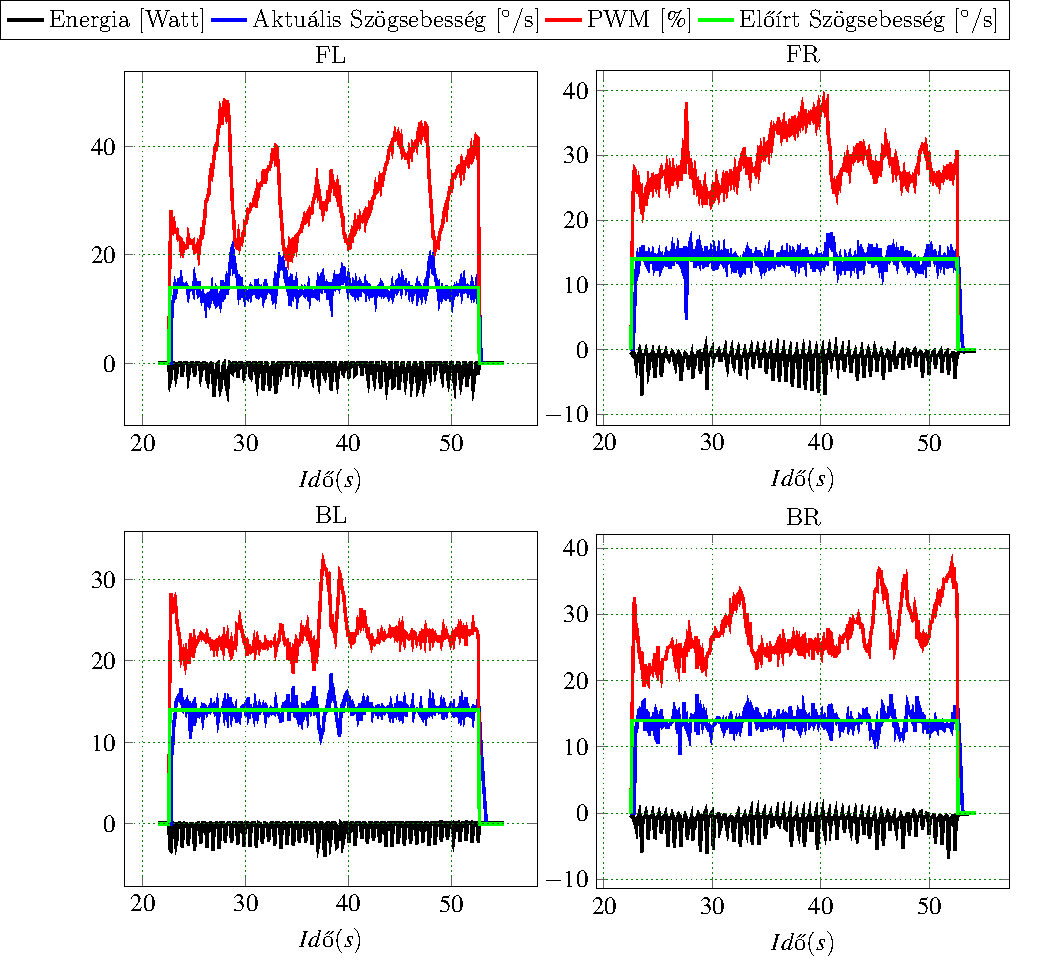
\includegraphics{tikz/LepcsoLexx.pdf}
  \caption{Lépcsőn lefele mozgás.}
  \label{fig:LepcsoLexx}
\end{figure}

A roboton IMU szenzora által mért értékek mutatják amint a $g=9.81 m/s^2$ gravitácios gyorsulás megjelenik a $aZ$ tengelyen \ref{fig:ImuLepcsoLe1}. Kezdetben a robot vizszinteshez közeli állapotban van X és Y.  A lépcson lefele mozgás során a $g$ fokozatosan átevődik az $aX$ tengelyre is amiatt, hogy a robot előre dől. A robot három lépcsőfokon halad át ami látható az ábrán is.

\begin{figure}[H]
  \begin{center}
  	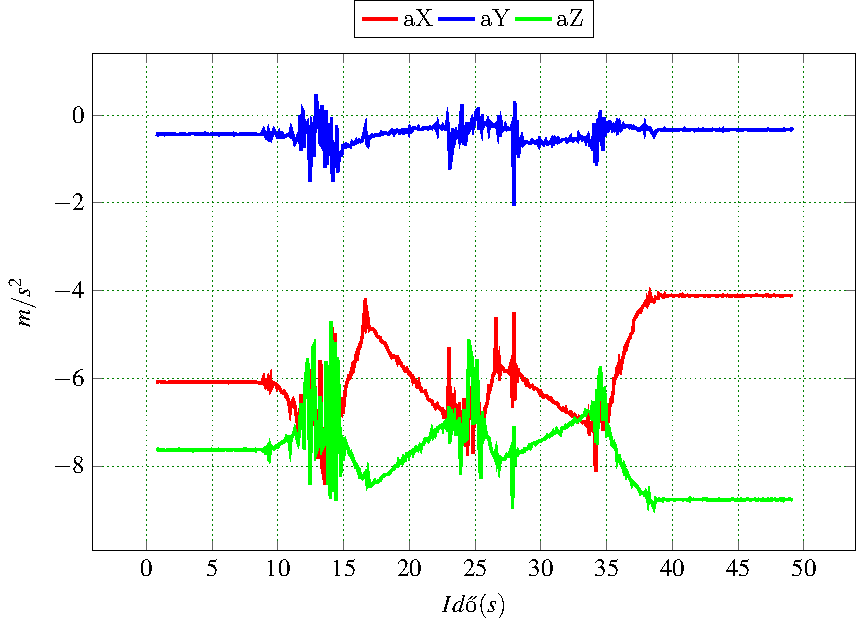
\includegraphics[scale=0.9]{tikz/ImuLepcsoLe1.pdf}
  \end{center}
  \caption{Lépcsön lefele mozgás, három lépcsőfok.}
  \label{fig:ImuLepcsoLe1}
\end{figure}

\begin{figure}[H]
  \begin{center}
  	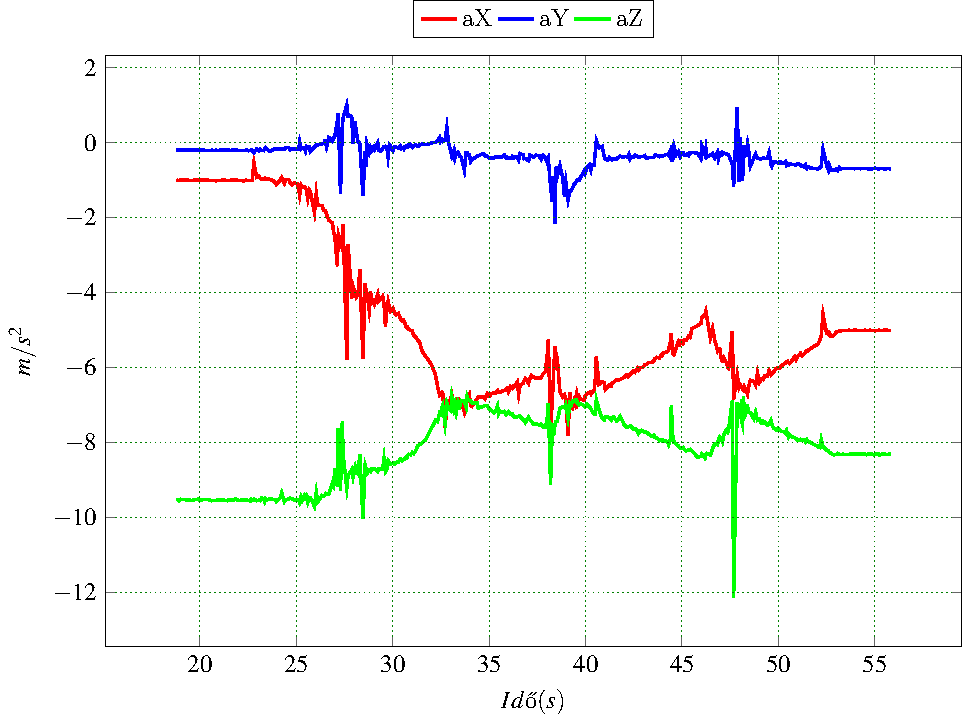
\includegraphics[scale=0.8]{tikz/ImuLepcsoFel1.pdf}
  \end{center}
  \caption{Lépcsőn felfele mozgás, kétlépcsőfok.}
  \label{fig:ImuLepcsoFel1}
\end{figure}

A lépcsőn felfele mozgás során a robot az előző állapotból indul visszafele. Azokban a pillanatokban, amikor a kerekek lecsúsznak a lépcső éléről, a kerekek szögsebessége megnő, mert a súrlódási erő lecsökken.  

Az \ref{fig:LepcsoFelxx} az $FL$ és $FR$ kerekeken nagyobb beavatkozó jel esik, amiatt hogy megnő a merőleges nyomóerő.

\begin{figure}[H]
  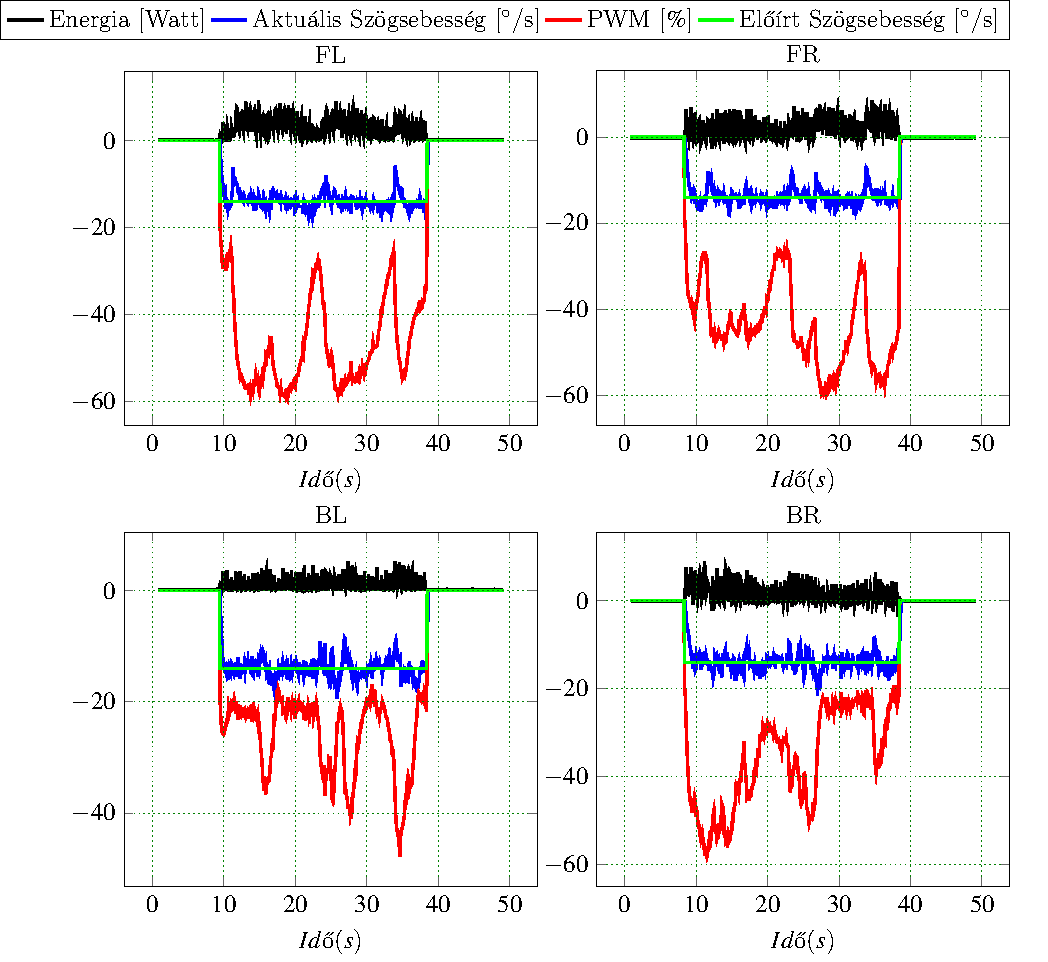
\includegraphics{tikz/LepcsoFelxx.pdf}
  \caption{Lépcsőn felfele mozgás}
  \label{fig:LepcsoFelxx}
\end{figure}

Abban az esetben ha a rontottal 90 \degree kisebb szög alatt közelítjük meg a lépcsőt akkor a robot mozgása a lépcsőn felfele könnyebben tud haladni. Ha a robot súlypontja a hátul  van és így közelítjük meg a lépcsőt megtörténhet az hogy a robot eleje elemelkedik és hátrabukik amiatt hogy a hátsó kerek beszorulnak a lépcsőfokba és a nyomaték így elemeli az első kerekeket.

Összevetve a \ref{fig:ImuLepcsoFel1} és a \ref{fig:ImuLepcsoAulaSlegenFel1}
látható hogy mindkét esetben az X és Y tengelyen tapasztaltunk bukdácsolást, ha 60\degree szög alatt közelítjük meg akkor az Y tengelyen is megjelenik egy dőlési szög.

A a pwm kitöltési tényezőjét tekintve az első kereke mindkét esetben nagyobb kitöltési tényezővel dolgoznak amiatt hogy a robot hattal megy fel a lépcsőn, a hátsó részben találhatóak az akkumulátorok.

\begin{figure}[H]
  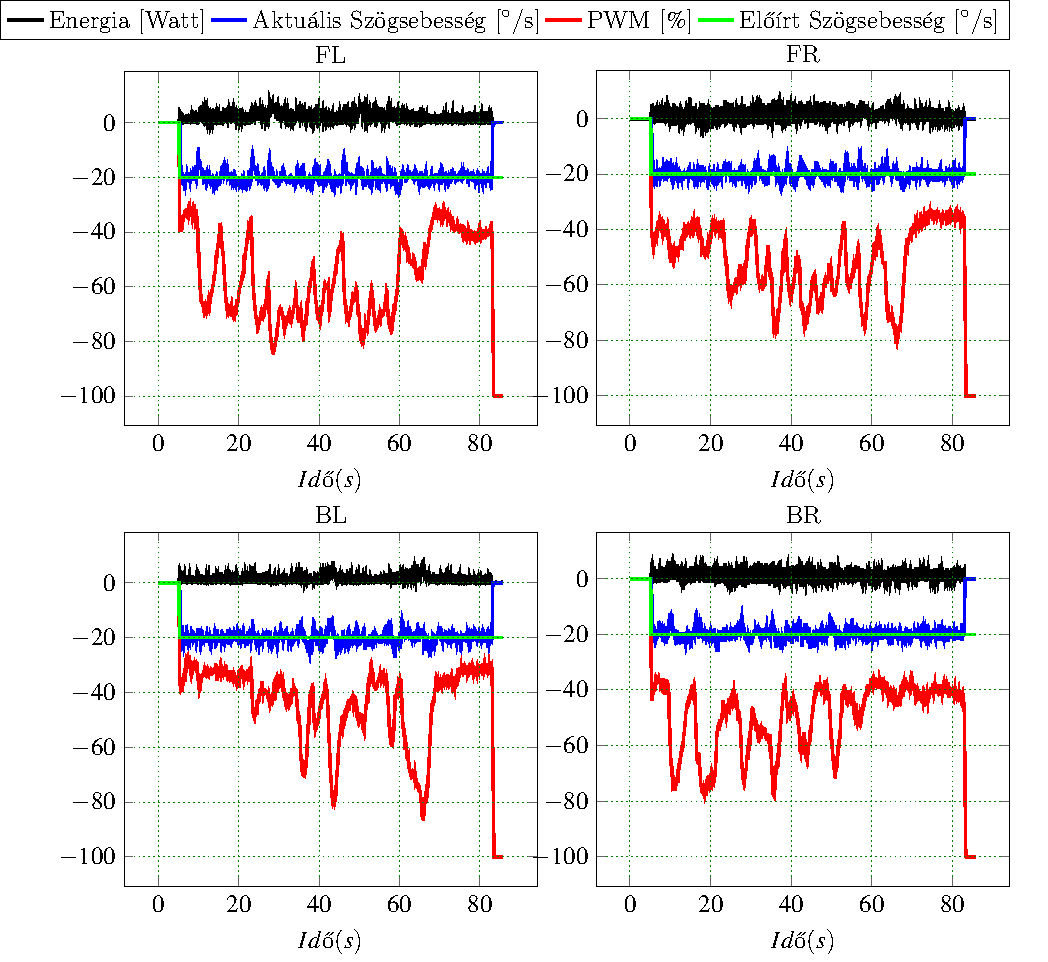
\includegraphics{tikz/LepcsoAulaSlegenFelx.pdf}
  \caption{Lépcsőn 60 \degree irányból felfele haladva 8 s.}
  \label{fig:LepcsoAulaSlegenFelx}
\end{figure}

\begin{figure}[H]
  \begin{center}
  	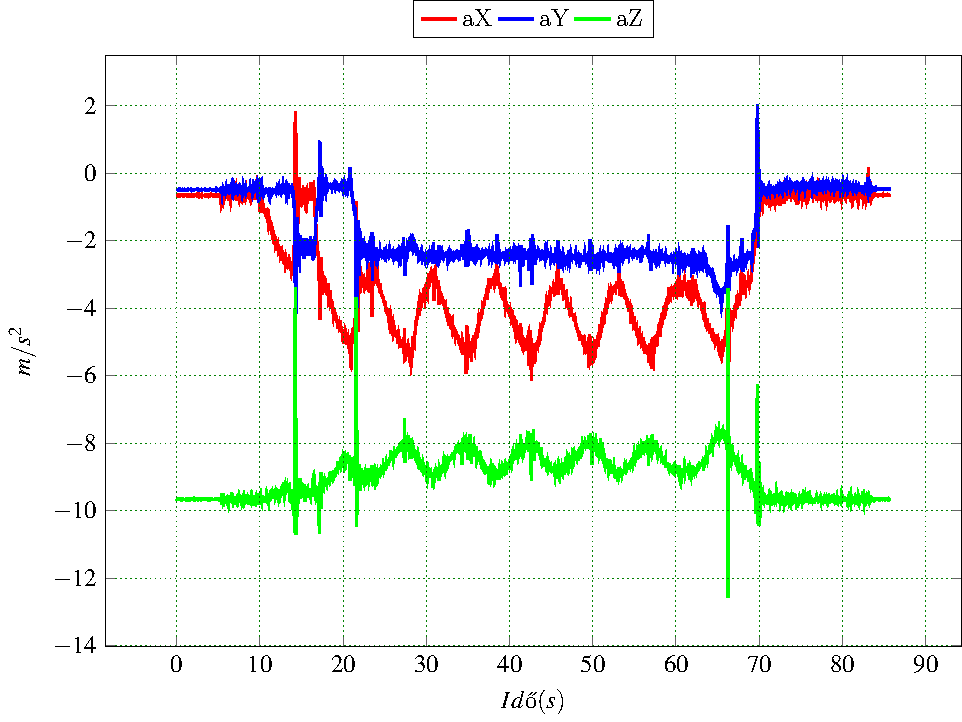
\includegraphics[scale=0.8]{tikz/ImuLepcsoAulaSlegenFel1.pdf}
  \end{center}
  \caption{Lépcsőn felfele mozgás 60 \degree szöget bezárva a lépcsőfokokkal.}
  \label{fig:ImuLepcsoAulaSlegenFel1}
\end{figure}















